\documentclass[a4paper, 11pt]{article}
\usepackage[spanish,es-tabla]{babel}
\usepackage[utf8]{inputenc}
\usepackage[hidelinks]{hyperref}
\usepackage[pdftex]{graphicx}
\usepackage{amsmath}
\usepackage{caption}
\usepackage{subcaption}
\usepackage{wrapfig}
\usepackage{titling}
\newcommand{\subtitle}[1]{%
  \posttitle{%
    \par\end{center}
    \begin{center}\large#1\end{center}
    \vskip0.5em}%
}
\title{Proyecto Final Curso Latex y Git Aplicado a la Investigación Científica}
\subtitle{Efecto de los vientos preponderantes en la
abundancia y biodiversidad de las comunidades de
elasmobranquios asociadas a arrecifes coralinos
en tres localidades de Nueva Caledonia}
\author{María Pozo Montoro}
\date{{Octubre 2018}}

\begin{document}
\vbox{
		\centering
		
\includegraphics[width=0.8\textwidth]{logoUGR}	
	\maketitle
	\thispagestyle{empty}
}
\newpage

\textit{Este texto corresponde a una reproducción parcial del Trabajo de Fin de Grado entregado en Junio 2018 por María Pozo Montoro con título Efecto de los vientos preponderantes en la abundancia y biodiversidad e las comunidades de elasmobranquios asociadas a arrecifes coralinos en tres localidades de Nueva Caledonia con el fin de evaluar los conocimientos adquiridos durante el curso de Latex y Git aplicado a la Investigación Científica mediante la elaboración de un Proyecto Final. Así pues el contenido y la bibliografía de este trabajo se encuentra incompletos.}
\thispagestyle{empty}

\newpage

\begin{abstract}
Repositorio del proyecto final: \url{https://github.com/mariapm295/proyecto_final.git} \\\\
La gran diversidad y aislamiento de los arrecifes coralinos de Nueva Caledonia permiten el desarrollo de una gran comunidad subacuática. Sin embargo, la misma remotidad que caracteriza al archipiélago provoca que en parte de su área no existan datos extensivos acerca de la abundancia y los patrones de distribución de ciertos organismos, en especial, de elasmobranquios, uno de los grupos de vertebrados más importantes y amenazados de nuestros océanos. Con el fin de recabar una mayor información acerca de la ecología de estos, en 2016 se realizó una expedición a las islas de Matthew y Walpole, así como a la zona del Cuerno Sur, como parte del proyecto Global FinPrint \url{https://globalfinprint.org/}, cuyo objetivo principal es determinar el estado de las poblaciones de elasmobranquios asociados a arrecifes coralinos de todo el mundo. Los datos se obtuvieron mediante la visualización y análisis de secuencias de vídeo tomadas mediante tecnología Baited Remote Underwater Video (BRUV), para responder a dos objetivos básicos: 1) identificar y comparar los patrones de distribución y abundancia entre las distintas áreas estudiadas, y 2) comprobar si, como sugirieron las observaciones preliminares efectuadas, existen diferencias en abundancia y diversidad entre zonas de barlovento y sotavento. La comparación de los valores de abundancia, riqueza y diversidad entre islas y lados de exposición al viento sugieren que las actividades humanas, presentes y pasadas, podrían haber modificado las comunidades más cercanas a los focos de población humanas, pese a la ausencia de una industria pesquera de elasmobranquios en la zona. Además, se pudo observar cómo el menor grado de exposición a los vientos preponderantes incrementó los valores de riqueza y diversidad de las comunidades de elasmobranquios en sotavento, ya sea por una mayor productividad o por un mayor gasto energético asociado a la zona de barlovento.\\\\

\textbf{Palabras clave:} BRUV, elasmobranquios, Nueva Caledonia, sotavento, tiburones.\\\\

\emph{Diseño del muestreo: Mark E. Bond y Michael R. Heithaus. Toma de datos en campo: Mark E. Bond. Extracción y análisis de datos: María Pozo Montoro. Redacción del Trabajo: María Pozo Montoro.}
\end{abstract}
\newpage

\tableofcontents
\listoffigures
\listoftables
\newpage

\section{Introducción}
Los elasmobranquios son una subclase de condrictios o peces cartilaginosos que incluye a más de 500 especies de tiburones y 630 de rayas \cite{Elbert2013}. El gran éxito evolutivo de este grupo les ha permitido adaptarse a una gran diversidad de ecosistemas marinos a lo largo de todos los océanos, desde las aguas tropicales del Pacífico oeste como Carcharhinus amblyrhynchos \cite{Wetherbee1997} hasta el ártico como Amblyraja hyperborea \cite{Lynghammar2012}, llegando a encontrase en ambientes batipelágicos de hasta 3600 metros de profundidad como Centroscymnus coelolepis. Algunas especies han llegado incluso a colonizar permanentemente cuerpos de agua dulce de Sudamérica, África, Australia, Sudamérica y el sudeste asiático como es el caso de Potamotrygon spp. o Glyphis spp. \cite{Martin2004}.
Muchas de estas especies ocupan altos lugares en las cadenas tróficas una vez superados los estadios juveniles vulnerables \cite{Compagno1990, Cortes1999}, lo que les otorga una importante función como reguladores top-down (“de arriba abajo”) de ecosistemas. Estos depredadores apicales son capaces de modificar el grado de depredación sufrido en niveles tróficos inferiores, modulando las poblaciones de depredadores más pequeños (mesodepredadores), mediante los efectos directos e indirectos de su consumo y el cambio comportamental y distribucional, ante el mayor riesgo de ser depredados \cite{Heithaus2004,Ritchie2009}. En la actualidad, varios estudios han presentado evidencias de las cascadas tróficas generadas al reducir las poblaciones de estas especies clave, precipitando la degradación de los ecosistemas y provocando incluso el colapso de industrias pesqueras por el aumento de las poblaciones de mesodepredadores, que llevan consigo el desequilibrio funcional de la cadena trófica \cite{Baum2003, Bascompte2005}. Así mismo, ecosistemas relativamente no perturbados como el atolón de Palmyra o las islas del Noroeste de Hawái presentan pirámides tróficas con una gran cantidad de elasmobranquios y otros depredadores apicales \cite{Friedlander2002,  Bradley2017}, mostrando ecosistemas más saludables y posiblemente más resilientes a perturbaciones que aquellos expuestos a la sobrepesca \cite{Sandin2008}. 
En la actualidad, el 17,4\% de las sólo 463 especies de elasmobranquios con suficientes datos para permitir su catalogación, se encuentran amenazadas según los criterios de la lista roja del IUCN \cite{Dulvy2014}. Considerando las especies clasificadas como Data Deficient (sin datos suficientes), este porcentaje podría aumentar hasta el 25\%, tratándose del grupo de vertebrados con menor número de especies no amenazadas \cite{Hoffmann2010}. Este declive se ha producido sobre todo como consecuencia de su sobrepesca para la obtención de carne y aletas, y la captura accidental de individuos que son posteriormente descartados o vendidos, dada la alta cotización en el mercado asiático de las aletas para la producción de la sopa de aleta de tiburón \cite{Dent2015, Dulvy2017}. Muchas especies de tiburones y rayas son especialmente vulnerables a esta sobreexplotación ya que presentan estrategias de organismos K, es decir, crecimiento lento, maduración tardía y número bajo de crías, haciendo que sus poblaciones tarden más tiempo en recuperarse en comparación con otras especies teleósteas de interés comercial \cite{Stevens2000}.
Dulvy et al. (2014) identificaron el Triángulo del Coral y el Mar Rojo como las regiones del planeta, junto con el Mar Mediterráneo, donde la biodiversidad de elasmobranquios se encuentra más comprometida. Sin embargo, la conservación de tiburones y rayas de arrecife, características de regiones tropicales y subtropicales, podría cumplir un papel vital para la protección de uno de los ecosistemas más amenazados desde finales del siglo XX. Los arrecifes de coral apenas ocupan entre un 0,1 y un 0,5\% de la superficie oceánica, pero albergan una de las mayores biodiversidades de nuestro planeta, con casi un tercio de las especies de agua salada encontradas en sus aguas. La sobrepesca, el aumento de las temperaturas por el cambio climático y la urbanización costera han provocado la pérdida de casi el 20% de los arrecifes de coral del planeta, y se calcula que para 2050 el porcentaje de arrecifes amenazados con desaparecer podría alcanzar casi el 100% siguiendo esta tendencia. Pese al actual debate acerca del rol funcional de los elasmobranquios en arrecifes coralinos, se ha sugerido que el mantenimiento de un buen estado de poblaciones de elasmobranquios podría incrementar la resiliencia de estos ecosistemas ante futuras amenazas, ya que:
\begin{enumerate}
\item Las especies de menor tamaño como el tiburón de puntas blancas de arrecife (Triaenodon obesus), el tiburón gris de arrecife (Carcharhinus amblyrhynchos) o la raya de Kuhl (Neotrygon kuhlii), incrementan la redundancia funcional de niveles tróficos intermedios \cite{Jacobsen2013, Frisch2016}, mitigando posibles cascadas tróficas ante la desaparición de especies con el mismo rol funcional. 
\item Las especies de gran tamaño como el tiburón tigre (Galeocerdo cuvier) o el tiburón martillo (Sphyrna lewini o Sphyrna mokarran) ejercen una regulación top-down del ecosistema, controlando las poblaciones de mesodepredadores \cite{Ruppert2013}, evitando de esta manera un consumo desproporcionado de las poblaciones de consumidores primarios, sin los cuales, se daría un crecimiento excesivo de algas que acabarían dominando el arrecife \cite{Bellwood2004}.
\end{enumerate}
Dada la creciente evidencia científica del papel de estas especies en el ecosistema y su alarmante desaparición, cada vez más naciones han comenzado a implementar diversas estrategias para promover la recuperación de sus poblaciones. A grandes rasgos, se pueden clasificar en dos tipos: regulaciones para una explotación sostenible y regulaciones para una restricción total de la pesca de elasmobranquios \cite{Shiffman2016}. Con el fin de determinar la efectividad de cada medida propuesta en su contexto, múltiples estudios se han centrado en comparar y valorar el estado de las comunidades de elasmobranquios sujetas a distintos grados de protección y presión antropogénica \cite{Juhel2018, Speed2018}. Sin embargo, el éxito de estas estrategias está ampliamente condicionado por el conocimiento actual de la biología de las especies en cuestión, siendo especialmente relevante determinar los factores que modulan su distribución y abundancia durante distintos estadios de vida \cite{Schlaff2014}.
Uno de los pasos críticos para diseñar un plan de conservación eficaz es conocer y predecir con exactitud dónde y cuándo se localizan las poblaciones de las especies vulnerables a la sobreexplotación \cite{Espinoza2014}. Los patrones de distribución de los elasmobranquios vienen determinados, como en otros grupos de organismos, por el conjunto de condiciones tanto abióticas como bióticas que maximizan. \textbf{(...)} Así mismo, recientemente Bangley et al. (2018) registraron el primer caso de una especie de tiburón que ha modificado su distribución como respuesta a los cambios globales en el clima asociados a las actividades humanas. Ante esta situación, es indispensable entender cómo y en qué medida diferentes factores ambientales modifican la distribución y supervivencia de estos organismos, ya que integrar este conocimiento, permitirá predecir de forma precisa el futuro de uno de los grupos de organismos más importantes y amenazados de los ecosistemas marinos. Por estas razones surge el objetivo del presente trabajo de fin de grado, que pretende caracterizar y comparar las comunidades de elasmobranquios de tres localidades relativamente inexploradas e intactas del archipiélago de Nueva Caledonia, con el fin de determinar los posibles efectos de los vientos preponderantes en sus niveles de abundancia y biodiversidad de elasmobranquios. Bajo este objetivo se plantean las siguientes hipótesis:
\begin{enumerate}
\item Esperamos un aumento significativo en la abundancia y diversidad de elasmobranquios en los arrecifes coralinos más antiguos, como consecuencia de un mayor desarrollo y complejidad de su arrecife.
\item Esperamos un aumento significativo en la abundancia y diversidad de las comunidades de elasmobranquios en los lados de barlovento (como consecuencia del mayor desarrollo coralino en zonas más expuestas al oleaje y pese al mayor gasto energético asociado a esta área) respecto a los de sotavento por el efecto de los vientos Alisios.
\end{enumerate}

\section{Estado del arte}

\subsection{Área de estudio}
\begin{figure}[b]
	
	\begin{subfigure}[b]{0.5\textwidth}
		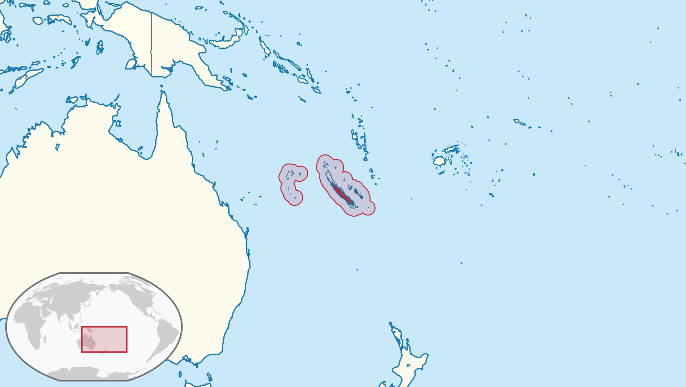
\includegraphics[width=\textwidth, height=35mm]{Mapa_Nueva_Caledonia}
		\caption{Ubicación de Nueva Caledonia}
		\label{fig:1.a}	
	\end{subfigure}
	\begin{subfigure}[b]{0.5\textwidth}
		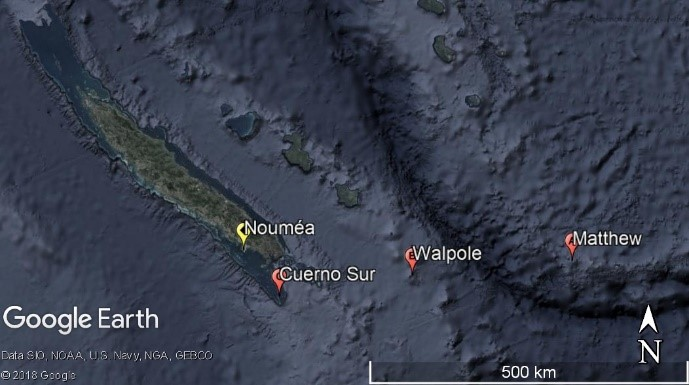
\includegraphics[width=\textwidth, height=35mm]{Mapa_area_de_muestreo}
		\caption{Vista satélite de las áreas de estudio}
		\label{fig:1.b}	
	\end{subfigure}
	\caption{Área de estudio}
\end{figure}

Las áreas de nuestro estudio pertenecen al archipiélago de Nueva Caledonia, localizado en el sudoeste del océano Pacífico (Figura \ref{fig:1.a}). Este territorio francés está incluido en la región biogeográfica del Indo-Pacífico Central, la cual constituye uno de los centros con mayor diversidad de nuestros océanos desde principios del Mioceno. 
Nueva Caledonia se encuentra formada por una serie de islas, casi todas ellas deshabitadas y  por la isla principal de Grande Terre, donde habitan 278.500 personas. Nueva Caledonia alberga en sus aguas el 27\% de la fauna ictiológica de Indo-Pacífico Central. Sus estructuras coralinas se caracterizan por poseer una alta diversidad, encontrándose entre ellas, la mayor barrera de coral del mundo con 1500 kilómetros de continuidad. Alrededor de 1,3 millones de $km^2$ de estas aguas se encuentran protegidas mediante el establecimiento de diversas figuras de protección. Además, la ausencia histórica de una industria pesquera de tiburones y la reciente prohibición de la pesca comercial y recreativa de estas especies en 2013 (decreto 2013-1007/GNC) proporcionan poblaciones relativamente intactas idóneas para contrastar nuestras hipótesis.
Durante aproximadamente el 70\% del año el archipiélago se encuentra expuesto a los intensos vientos Alisios, procedentes del sudeste por la circulación de Walker. Estos regímenes de vientos resultan idóneos para comprobar su posible efecto modelador en las comunidades elasmobranquias. Además, nuestras áreas de estudio se ven afectadas por la Corriente Sur Ecuatorial, que al llegar a Nueva Caledonia se divide formando la Corriente de Nueva Caledonia Norte y la Corriente de Nueva Caledonia Sur . La temperatura media en superficie es de 27 a 28 ºC en verano y de 23 a 25 C en el invierno austral. La salinidad varía entre los 35,4 y los 35,8 PSU a lo largo del año. Durante nuestro periodo de estudio la temperatura fue estable entre las distintas zonas con una media de 24,5 C.

\subsection{Selección de zonas}
El presente estudio comprende tres localizaciones (Figura \ref{fig:1.b}) cuyos arrecifes coralinos presentan distintos grados de desarrollo en función de su antigüedad. Además, dada su remotidad, los datos obtenidos de Matthew y de Walpole son de los primeros obtenidos sobre las comunidades de elasmobranquios de estas localizaciones.

\subsubsection{Isla de Matthew}
La isla de Matthew (22º 20,574’S, 171º 21,308’ E) se trata de una joven isla volcánica de unos 0,7 km2 (Figura 2) situada a 300 km de la Grande Terre. Se encuentra formada por dos conos volcánicos unidos por un istmo. El cono oeste se formó en 1949 y la última erupción volcánica confirmada es de 1958. La isla continúa presentando actividad sísmica, así como volcánica en forma de emisiones de gas sulfuro, procedentes del cono oeste que incrementan la turbidez del agua y modifican su pH. Su sistema coralino es el más joven y menos desarrollado, conformado únicamente por las colonias coralinas aisladas que son capaces de sobrevivir la turbidez y las emisiones de gases. Forma parte del Parque Natural del Mar de Coral.
\subsubsection{Isla de Walpole}
La isla de Walpole (22º 35,897’S, 168º 57,156’ E) se trata de una isla de origen volcánico de unos 2,0 km2 (Figura 3) situada a 180 km de la Grande Terre. Se encuentra constituida por una meseta plana delimitada por acusados precipicios, a causa de la erosión del viento y repetidos hundimientos durante los últimos 400.000 años. Desde 1910 a 1936 vivieron unas 300 personas en la isla que extrajeron más de 100.000 toneladas de guano; sin embargo, en la actualidad se encuentra deshabitada. Posee un desarrollado arrecife costero con una edad intermedia de unos 125.000 años de antigüedad. Como Matthew, forma parte del Parque Natural del Mar de Coral. 

\subsubsection{El Cuerno Sur de la Gran Laguna Sur}
El Cuerno sur de la Gran Laguna Sur (22º 55,960’S, 166º 59,607’ E) es una barrera de coral externa (Figura 4) que delimita la Gran Laguna Sur, la cual posee unos 2000 km2. Se encuentra a una distancia de entre 5 a 40 km de la Grande Terre en función de la zona. El oeste de la barrera presenta 6 canales profundos de unos 60 metros de profundidad que conectan la Laguna con el Mar de Coral. Así mismo, durante regímenes intensos de los vientos Alisios, especialmente de Octubre a Abril, se dan fenómenos de afloramiento de aguas profundas que enfrían el agua unos 5ºC e incrementan la productividad. Se trata del sistema coralino más antiguo y diverso de nuestro estudio, calculándose que comenzó a formarse hace unos 900.000 años. La Gran Laguna Sur y sus distintos hábitats se encuentran protegidos como patrimonio de la humanidad de la UNESCO, sin embargo, continua viéndose afectada por las actividades humanas procedentes de la isla principal, especialmente por la industria minera del níquel y del cromo. 

\subsection{Método de censo}
Los datos fueron obtenidos usando tecnología Baited Remote Underwater Video (en adelante BRUV) durante la expedición del 23 de Junio al 1 de Julio de 2016 en el buque de investigación Amborella. Esta expedición fue motivada por el Global FinPrint Project \url{https://globalfinprint.org/}, que tiene como objetivo examinar y comparar el estado de las poblaciones de tiburones de arrecifes por todo el globo. La ventaja de la técnica BRUV respecto a otros métodos de muestreo tradicionales es el reducido impacto ecológico, coste y tiempo requerido para la toma de datos en campo.  Así mismo, se ha podido comprobar que los datos de abundancia y riqueza obtenidos mediante BRUV son aceptablemente equiparables a los obtenidos mediante censo visual y captura de individuos para estas especies. Por lo tanto, en la actualidad, se trata de una metodología ampliamente utilizada para el estudio de su ecología y comportamiento \cite{Juhel2018, Speed2018}.
\begin{wrapfigure}{r}{0.5\linewidth}
    \centering
    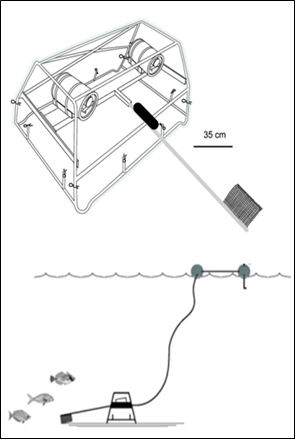
\includegraphics[width=0.5\textwidth]{BRUV.png}
    \caption{\textbf{Arriba: }Diseño BRUV. \textbf{Abajo: }Esquema de colocación de BRUV}{{\footnotesize Fuente: (Harley et al 2013)}}
    \label{fig:2}
\end{wrapfigure}
Cada BRUV estaba formado por dos cámaras GoPro HD HERO2 montadas en un soporte de metal, al cual se unían 3 barras de PVC de 1,5 m de longitud, cuyo extremo final poseía un cebo (1 kg de sardinas trituradas) contenido en una malla de metal, dentro del ángulo de visión de las cámaras (Figura 5). Se colocaron un total de 109 BRUVs (29 en Matthew, 40 en Walpole y 40 en el Cuerno Sur) escogidos previamente de manera aleatoria para cubrir la superficie de las distintas áreas de estudios. Cada BRUV se colocó durante el día a una profundidad de entre 44 y 15 metros grabando 60 minutos de vídeo, desde el momento que quedaba adecuadamente colocado en el fondo hasta que se recogía, mediante el uso de un motor que cobraba el cabo que unía el BRUV a una boya para su relocalización (Figura 5). Con el fin de evitar interacciones durante la colocación y recogida, la distancia mínima entre dos BRUVs consecutivos fue de 200 metros. Además, al principio de cada colocación se midió la temperatura del agua y la profundidad a la que quedaba colocado el BRUV mediante una sonda Lowrance XD85. 
Dada la topología de la isla de Matthew no se pudieron colocar BRUVs en la zona sur, por la caída a grandes profundidades de sus fondos. Las complicadas e inusuales condiciones meteorológicas impidieron continuar con el muestreo planeado al sudoeste del Cuerno Sur, disponiendo únicamente de 4 BRUVs de la zona de sotavento. Decidimos no excluir el Cuerno Sur de nuestro análisis dado el posible valor de la información extraída para futuros estudios en la zona. Sin embargo, sí que eliminamos aquellos vídeos en los que el BRUV quedaba mal colocado, así como cuando la visibilidad se veía comprometida por las emisiones de la isla de Matthew, ya que tras su visualización se pudo comprobar que la probabilidad de detección de organismos en estos se veía muy reducida. En conjunto, los datos utilizados en este estudio provienen de 96 BRUVs útiles.
Para la extracción de datos, un único anotador experimentado visualizó los vídeos obtenidos por la cámara derecha a velocidad x1. Se identificó la especie de cada elasmobranquio capturado en cámara y se estableció la abundancia relativa de cada una por BRUV mediante el conteo del número máximo de individuos de una misma especie en un fotograma durante una hora de vídeo (MaxN). Esta medida permite la estandarización del conteo, con el fin de comparar los datos entre distintas localizaciones, mientras que se evita sobreestimar la abundancia relativa al contar más de una vez los individuos que pasan por delante de la cámara reiteradas veces. La identificación y nomenclatura utilizada sigue a Elbert et al. (2013) y Allen et al. (2015).\\
\begin{table}[htbp]
\begin{center}
\begin{tabular}{|c|c|c|c|}
\hline
 & Sotavento & Barlovento & Total\\
\hline
Matthew & 15 & 14 & 29\\
Walpole & 20 & 20 & 40\\
Cuerno Sur & 34 & 6 & 38\\
\hline
\end{tabular}
\caption{Número de BRUV's por localidad y lado}
\label{tabla:1}
\end{center}
\end{table}

\subsection{Análisis de los datos}
Los datos obtenidos se tabularon en una hoja de cálculo de Microsoft Excel (2017) especificando las siguientes variables: el identificador alfanumérico único de cada BRUV, la localización en la que se colocaba (Matthew, Walpole o Cuerno Sur), el lado (Barlovento, Sotavento), las coordenadas GPS exactas de su posición en grados minutos decimales, el momento del día en el que se colocaba (mañana o tarde), la fecha, la temperatura durante la colocación y la recogida del BRUV, la profundidad a la que quedaba colocado y el MaxN de cada especie de la zona.
Una vez introducidos los datos se procedió a calcular la abundancia relativa total (Sumatoria del MaxN de todas las especies capturadas durante un BRUV, Fórmula \ref{CumMaxN}), la riqueza (Número de especies presentes en cada BRUV, Fórmula \ref{Richness}) y la diversidad mediante Índice de Shannon (Fórmula \ref{Shannon}). Para este último, se eliminaron aquellos BRUV en los que no se detectó ninguna especie.
A continuación, se importó esta hoja de cálculo al software R (R Core Team). Previamente a los análisis, se comprobó si las condiciones de la prueba ANOVA, es decir, normalidad, homocedasticidad, independencia y balanceo se cumplían para nuestros datos. Un análisis gráfico preliminar indicó una distribución asimétrica a la izquierda de nuestros datos alejada de una distribución normal, lo cual se comprobó mediante un test de Shapiro-Wilk, considerado más robusto para datos con distribución asimétrica. Así mismo la homogeneidad de varianzas se comprobó mediante un test de Levene basado en la mediana o también llamado test de Brown-Forsythe, también más robusto con datos con asimetría hacia la izquierda. Para cada variable se usaron como clasificadores “Localización” y “Lado”. Las varianzas fueron homogéneas en todos los casos. Por el contrario, en ninguno de los casos la distribución fue normal. Se trató de normalizar los datos siguiendo las transformaciones habituales sin surgir efecto alguno, posiblemente debido a la naturaleza de los datos que responde a los de tipo conteo con una asimetría hacia la izquierda. Por otro lado, mientras que el diseño de muestreo aseguró la independencia de los datos, los contratiempos durante la expedición anteriormente expuestos dieron lugar a un menor número de BRUVs en el lado de sotaveto del Cuerno Sur, comprometiendo el balanceo.
Dada la ausencia de normalidad, así como de balanceo en las muestras entre barlovento y sotavento del Cuerno Sur, se procedió al análisis comparativo de las variables calculadas en función de la localización y el lado mediante el test Scheirer-Ray-Hare. Este test se trata de una extensión del test de Kruskal-Wallis por rangos, siendo el equivalente no paramétrico a un ANOVA de dos factores. En aquellos casos en los que el test mostró significación para el factor “Localización” (p$<$0.05), se procedió a la realización de un test post-hoc para determinar qué grupos en este factor mostraban diferencias significativas. Para ello, utilizamos la prueba U de Mann Whitney entre las distintas combinaciones de localizaciones con corrección de Bonferroni-Holm, con el fin de hacer frente a la inflación del error Tipo I asociado a un mayor número de comparaciones.

\begin{equation}
\label{CumMaxN}
Cumulative\: MaxN = \sum_{i=1}^9MaxN=MaxN_{Especie_{1}} + ... + MaxN_{Especie_{9}}
\end{equation}

\begin{equation}
\label{Richness} 
Riqueza\:de\:especies  = \sum\:Especies = Especie_{1} + Especie_{2} + ...
\end{equation}

\begin{equation}
\label{Shannon}
\begin{split}
H' & =-\sum_{i=1}^9p_{Especie_{i}}\; lnp_{Especie_{i}}\\\\
p_{Especie_{i}} & = \frac{MaxN_{Especie_{i}}}{Cumulative MaxN}
\end{split}
\end{equation}

\bibliographystyle{unsrt}
\bibliography{ProyectoFinal}
\end{document}